%% frontier_mpf.tex — Operator Lightcone Wavemap
%%
%% Build: pdflatex frontier_mpf.tex && bibtex frontier_mpf && pdflatex frontier_mpf.tex
%%
%% Shell: PaperHeavyHex/heavyhex.tex

\documentclass[12pt]{article}
\usepackage[top=2cm,bottom=2cm,left=1.5cm,right=1.5cm,columnsep=0.5cm]{geometry}
\usepackage{graphicx}
\usepackage{amsmath,amssymb}
\usepackage{bm}
\usepackage{hyperref}
\usepackage{booktabs}
\usepackage{xcolor}
\usepackage{microtype}
\usepackage{abstract}
\usepackage{tikz}
\usetikzlibrary{positioning,shapes.geometric,decorations.pathreplacing}
\renewcommand{\abstractnamefont}{\normalfont\bfseries}
\renewcommand{\abstracttextfont}{\normalfont\small}

%% TODO markers
\newcommand{\TODO}[1]{\textcolor{red}{\textbf{[TODO: #1]}}}
\newcommand{\CITE}[1]{\textcolor{blue}{[#1]}}
\newcommand{\chimax}{\chi_{\max}}

\begin{document}

\title{Site-Centric Operator Wavefront as a Spatial Observable\\
       for Noise-Amplified Tensor Network Simulation}

\author{
 Paolo D'Alberto\thanks{Advanced Micro Devices, Inc. (AMD).
 \texttt{paolo.dalberto@amd.com}.
 This work was developed in active collaboration with Claude (Anthropic).}\\
 \small Advanced Micro Devices, Inc.\\
 \small\texttt{paolo.dalberto@amd.com}
}

\date{\today}

% ─────────────────────────────────────────────────────────────────────────────
\maketitle

\begin{abstract}
We introduce a site-centric wavefront analysis for operator spreading in
noisy quantum lattice simulations.
Running noiseless and noisy Trotter evolution at noise amplification factors
$\gamma \in \{1,2,3\}$, we assign each lattice site $v$ two natural observables:
the \emph{arrival delay} $l_\gamma(v) = t_\gamma(v) - t_{\rm nl}(v)$
(how many cycles later the noisy wave crosses threshold compared to noiseless)
and the \emph{natural ratio}
$r_\gamma(v) = n_{\gamma}(v,\, t_\gamma(v)) \,/\, n_{\rm nl}(v,\, t_\gamma(v))$
(how much the noiseless wave has grown at site $v$ by the time the noisy wave arrives).
Together these form a \emph{wavemap} — a spatial portrait of noise effects
across the lattice, with each site receiving a single delay and ratio value
per noise level.
We demonstrate on two topologies: an IBM heavy-hex $3\times3$ lattice
with per-bond hardware characterization noise and a rectangular $7\times7$
lattice with synthetic depolarizing noise.
Eigenvalue analysis of the composed Pauli transfer matrices confirms that
in both cases the noise channel is a near-diagonal damping operator
(off-diagonal power $< 0.1\%$), and the Pauli mixing structure is entirely
from the gate ($\sim 36\%$ off-diagonal power, independent of $\gamma$).
Noise acts as a pure amplitude suppression: it delays the wavefront by
slowing threshold crossing, and the ratio $r_\gamma(v)$ encodes the
cumulative damping along each propagation path from center to $v$.
The wavemap connects to the multi-product formula (MPF): the delay field
$l_\gamma(v)$ is a spatial version of the temporal error, and the
Lieb-Robinson bound $F_{\rm nl}(t)$ provides a causal ceiling for
MPF-corrected frontier recovery.
\end{abstract}

% ─────────────────────────────────────────────────────────────────────────────
\section{Introduction}
\label{sec:intro}

The operator lightcone describes the causal structure of quantum information
spreading under local Hamiltonian evolution~\cite{liebrobinson1972}.
For a local observable $O_c$ initialized at site $c$, the Heisenberg-picture
operator $O_c(t) = e^{iHt}O_c e^{-iHt}$ acquires support at progressively
more distant sites as $t$ grows.
The non-identity Pauli weight $n(v,t)$ — the fraction of the operator
living on site $v$ at cycle $t$ — is a direct measure of this spreading.

Classical tensor network simulators can compute $n(v,t)$ for small systems
via Pauli transfer matrices~\cite{TODO}, enabling quantitative comparison
between noiseless and noisy dynamics.
The \emph{frontier} of the spreading wave defines a frontier velocity
$v_{\rm hop}$ that calibrates both the Hamiltonian and the simulation
fidelity~\cite{dalberto2026cppsim}.

Hardware quantum processors introduce noise channels between gate
applications. The central question for quantum error mitigation is:
how does this noise deform the operator spreading?
If the noise is a simple amplitude suppression (diagonal Pauli transfer matrix),
it delays the wavefront and damps its amplitude but does not change the
spatial structure of propagation — a calibration problem.
If it introduces Pauli mixing (off-diagonal terms), it scrambles the
propagation pattern — a fundamentally harder problem.

In this paper we show, via direct eigenvalue analysis of the composed
gate-plus-noise Pauli transfer matrices, that both IBM hardware noise
and synthetic depolarizing noise belong to the first category:
the noise channel is a near-diagonal damping operator, and all
Pauli mixing is due to the gate.
This observation motivates a site-centric wavefront analysis that cleanly
separates the two effects: delay (noise-induced timing shift) and damping
ratio (noise-induced amplitude suppression).

The resulting \emph{wavemap} assigns each site $v$ a single delay
$l_\gamma(v)$ and ratio $r_\gamma(v)$ per noise level $\gamma$,
forming a spatial portrait of noise effects across the lattice.
We demonstrate this on two topologies and connect the wavemap to the
Lieb-Robinson-constrained spatial multi-product formula (MPF).

% ─────────────────────────────────────────────────────────────────────────────
\section{Setup}
\label{sec:setup}

\subsection{Model and simulation}
\label{sec:model}

We simulate the kicked isotropic Heisenberg model in the Heisenberg picture:
\begin{equation}
    H = J \sum_{\langle ij\rangle} \bigl(X_iX_j + Y_iY_j + Z_iZ_j\bigr),
    \qquad
    U_{\rm kick} = \prod_v R_x(2\phi)_v,\quad \phi = 1.41371669
\end{equation}
with per-bond coupling $J_{\langle ij\rangle}$ from device characterization
and Trotter step $\varepsilon = 0.10$.
We use CppSim~\cite{dalberto2026cppsim}, a GPU-accelerated belief propagation
tensor network simulator.
Operators are evolved via $16\times16$ real Pauli transfer matrices (PTMs);
bond dimension $\chi$ is controlled by Householder QR truncation at cutoff $\delta$.
The non-identity Pauli weight at site $v$ is $n(v,t) = \sum_{d\in\{X,Y,Z\}}\langle P_d^{(v)}\rangle$.
All results use $\varepsilon=0.10$, $\delta=10^{-3}$, output precision $10^{-7}$
(7 decimal places), and threshold $\varepsilon_{\rm th}=10^{-4}$.

\subsection{Noise models}
\label{sec:noise}

\paragraph{Heavy-hex hardware noise.}
Per-bond, per-color-class $16\times16$ PTMs are measured from device
characterization data (ibm\_basquecountry).
The composed noisy bond PTM is:
\begin{equation}
    \mathrm{PTM}_{\rm noisy}^{(b)} =
    G_1 \cdot M_\gamma^{(b)} \cdot G_2(\alpha_b) \cdot M_\gamma^{(b)}
    \cdot G_3(\alpha_b) \cdot M_\gamma^{(b)} \cdot G_4(\delta_b)
    \label{eq:noisy_ptm}
\end{equation}
where $M_\gamma^{(b)} = \gamma M_{\rm hw}^{(b)} + (1-\gamma)I$ linearly
amplifies the hardware noise channel, and $G_1\ldots G_4$ implement the
hardware gate decomposition.

\paragraph{Synthetic depolarizing noise (rect $7\times7$).}
Rows $1\ldots15$ of the ideal bond PTM $G^{(b)}$ are scaled by $(1-p\gamma)$
with $p=0.01$:
\begin{equation}
    \mathrm{PTM}_{\rm noisy}^{(b)}[i,j] = \begin{cases}
        G^{(b)}[0,j] & i=0 \\
        (1-p\gamma)\,G^{(b)}[i,j] & i \geq 1
    \end{cases}
    \label{eq:dep_ptm}
\end{equation}
This is the depolarizing channel composed with the gate:
all non-identity output Pauli components are uniformly damped by $(1-p\gamma)$.

\begin{figure}[t]
\centering
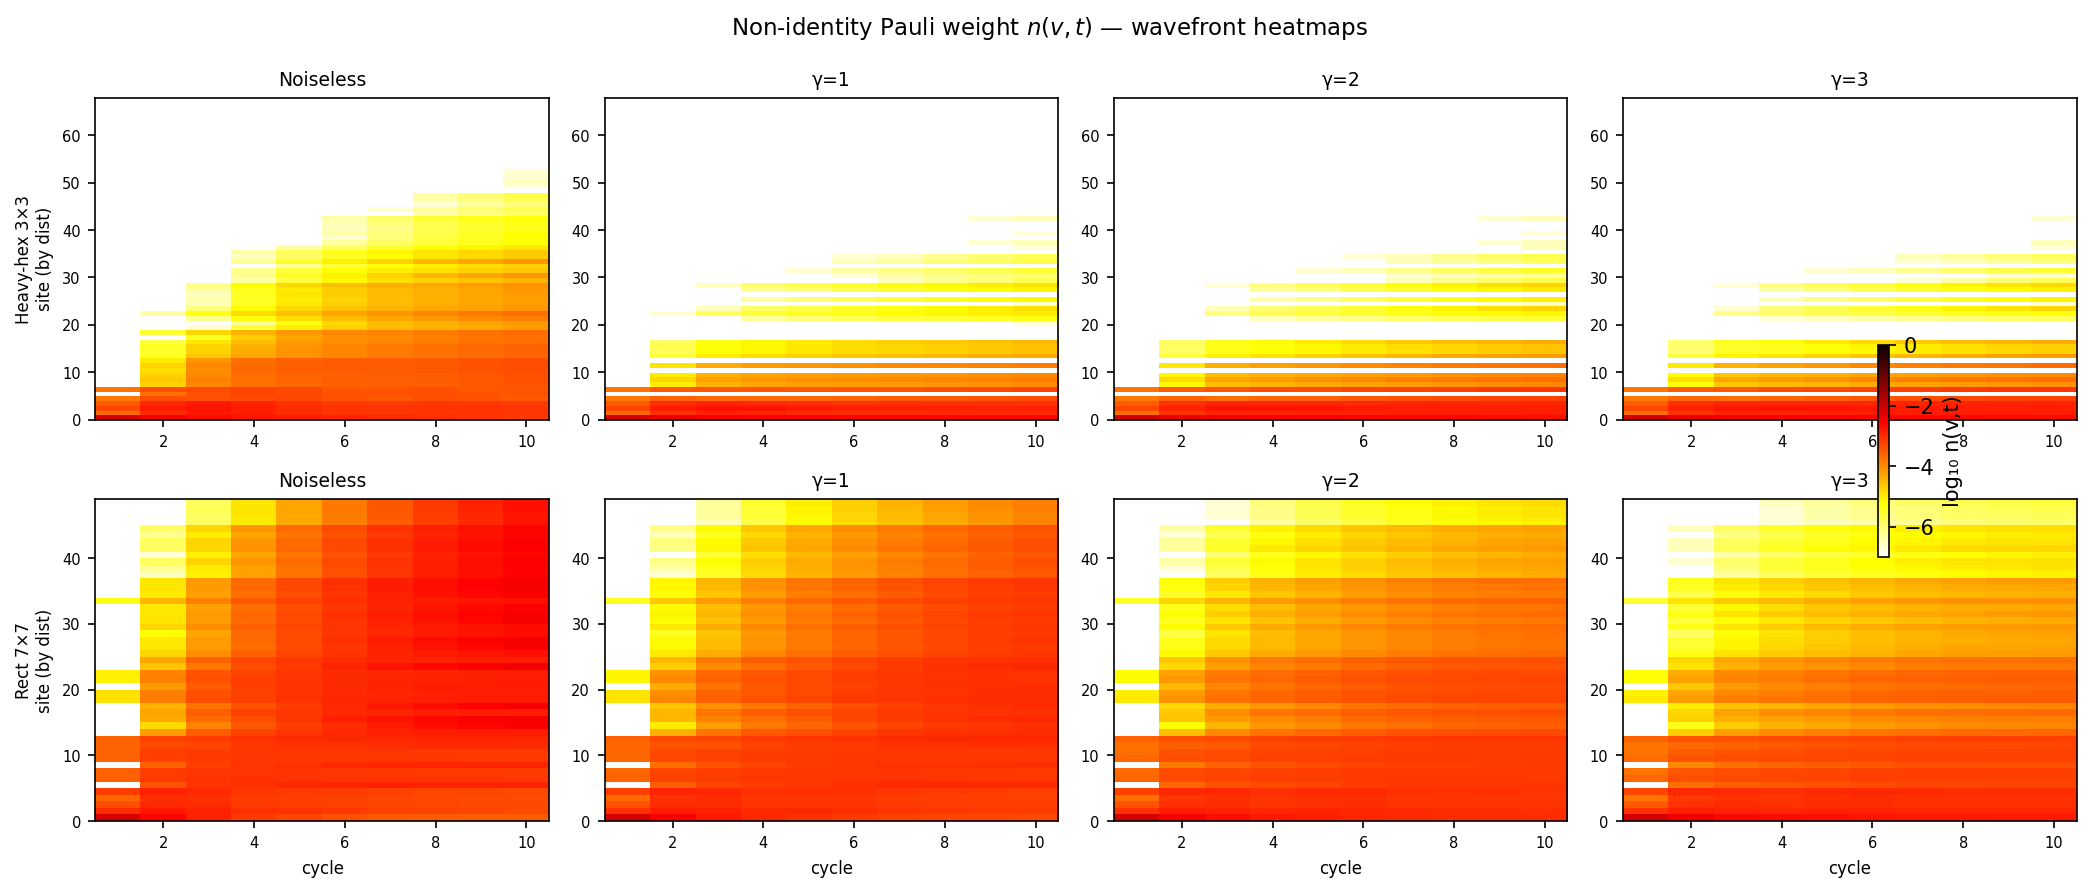
\includegraphics[width=\columnwidth]{fig_lightcone_heatmap.png}
\caption{Non-identity Pauli weight $n(v,t)$ per site per cycle for noiseless (NL)
and three noise levels ($\gamma=1,2,3$) on the heavy-hex $3\times3$ lattice
(left) and rect $7\times7$ (right), both initialized at the center site.
Color encodes $\log_{10} n(v,t)$; white = below threshold.
The wavefront advances diagonally in the (space, time) plane at velocity $v_{\rm hop}$.
Noise suppresses amplitudes, pushing the threshold-crossing later — a uniform
shift of the wavefront, not a change of its spatial pattern.}
\label{fig:heatmap}
\end{figure}

\subsection{Eigenvalue analysis of the composed PTMs}
\label{sec:eig}

Before defining the wavefront observables, we establish the noise character
by direct eigenvalue analysis of the HPP-compiled composed PTMs.

\begin{table}[h]
\centering
\small
\begin{tabular}{l r rr r r}
\toprule
Configuration & Bonds & Off-diag frac. & $\max|\mathrm{Im}(\lambda)|$
              & $n(\mathrm{Re}<0)$ & $n(|\lambda|>1)$ \\
\midrule
Heavy-hex ideal    & 76 & 0.357 & 0.964 & 0  & 0 \\
Heavy-hex $\gamma=1$ & 76 & 0.356 & 0.950 & 0  & 0 \\
Heavy-hex $\gamma=2$ & 76 & 0.355 & 0.950 & 2  & 0 \\
Heavy-hex $\gamma=3$ & 76 & 0.355 & 0.950 & 2  & 0 \\
\midrule
Rect $7\times7$ ideal    & 84 & 0.360 & 0.891 & 0  & 0 \\
Rect $7\times7$ $\gamma=1$ & 84 & 0.360 & 0.882 & 0  & 0 \\
Rect $7\times7$ $\gamma=2$ & 84 & 0.360 & 0.873 & 0  & 0 \\
Rect $7\times7$ $\gamma=3$ & 84 & 0.359 & 0.865 & 0  & 0 \\
\bottomrule
\end{tabular}
\caption{Eigenvalue statistics of composed noisy PTMs across all bonds.
Off-diagonal fraction = off-diagonal power / total power (averaged over bonds).
The off-diagonal fraction is \emph{constant across $\gamma$} in both topologies
($\Delta < 0.002$), confirming that Pauli mixing is entirely from the gate.
The noise channel contributes only uniform diagonal damping.
The 2 negative eigenvalues at $\gamma=2,3$ in heavy-hex are at $\mathrm{Re}=-10^{-5}$
— numerical precision, not a structural change.}
\label{tab:eig}
\end{table}

Table~\ref{tab:eig} establishes the key result: the off-diagonal fraction is
constant across $\gamma$ ($\Delta < 0.002$) in both topologies.
Noise adds no rotation structure; it only scales eigenvalue magnitudes.
All Pauli mixing comes from the gate $G$.
This means:
\begin{itemize}
    \item The noise channel is a \emph{pure damping operator} at the PTM level
    \item The spatial propagation pattern of the operator is \emph{determined
          by the gate}, not the noise
    \item Noise delays the wavefront by reducing amplitudes below threshold;
          it does not redirect propagation
\end{itemize}

% ─────────────────────────────────────────────────────────────────────────────
\section{Site-Centric Wavefront Observables}
\label{sec:observables}

\subsection{Arrival times and delay}
\label{sec:delay}

For each site $v$ we define the \emph{arrival time} as the first cycle at
which the wave crosses threshold:
\begin{equation}
    t_\gamma(v) = \min\bigl\{t : n_\gamma(v,t) > \varepsilon_{\rm th}\bigr\}
    \label{eq:arrival}
\end{equation}
with $t_\gamma(v) = \infty$ if the wave never arrives within the simulation window.
The \emph{arrival delay} is:
\begin{equation}
    l_\gamma(v) = t_\gamma(v) - t_{\rm nl}(v)
    \label{eq:delay}
\end{equation}
defined only for sites where both $t_{\rm nl}(v)$ and $t_\gamma(v)$ are finite.
Since the noise is a pure amplitude damping, it reduces $n_\gamma(v,t)$ below
$n_{\rm nl}(v,t)$ at every site and cycle.
The threshold $\varepsilon_{\rm th}$ is crossed later by the noisy wave,
giving $l_\gamma(v) \geq 0$ always.

\subsection{Natural amplitude ratio}
\label{sec:ratio}

At the moment $t_\gamma(v)$ when the noisy wave just crosses threshold at $v$:
\begin{itemize}
    \item $n_\gamma(v,\, t_\gamma(v)) \approx \varepsilon_{\rm th}$
          — the noisy wave just arrived
    \item $n_{\rm nl}(v,\, t_\gamma(v)) \gg \varepsilon_{\rm th}$
          — the noiseless wave has been growing at $v$ for $l_\gamma(v)$ cycles
\end{itemize}
The \emph{natural ratio} is:
\begin{equation}
    r_\gamma(v) = \frac{n_\gamma(v,\; t_\gamma(v))}{n_{\rm nl}(v,\; t_\gamma(v))}
    \label{eq:ratio}
\end{equation}
This ratio has a clean physical interpretation.
Since the noise damps all Pauli components uniformly along each bond,
a site at BFS distance $d$ reached via a path of $N$ gate applications
accumulates a total damping factor $(1-p\gamma)^N$ (for depolarizing) or
$\prod_e \lambda_{\rm min}^{(e)}(\gamma)$ (for hardware noise).
The noiseless wave, meanwhile, has grown at $v$ for $l_\gamma(v)$ extra cycles.
The ratio $r_\gamma(v) < 1$ measures the combined effect:
path-dependent cumulative damping amplified by the extra growth time of the
noiseless wave.

Crucially: $r_\gamma(v) \leq 1$ always (the noiseless wave is always larger
at $t_\gamma(v) \geq t_{\rm nl}(v)$), and $r_\gamma(v) \to 1$ when $l_\gamma(v) = 0$
(simultaneous arrival, no damping effect visible).

\begin{figure}[t]
\centering
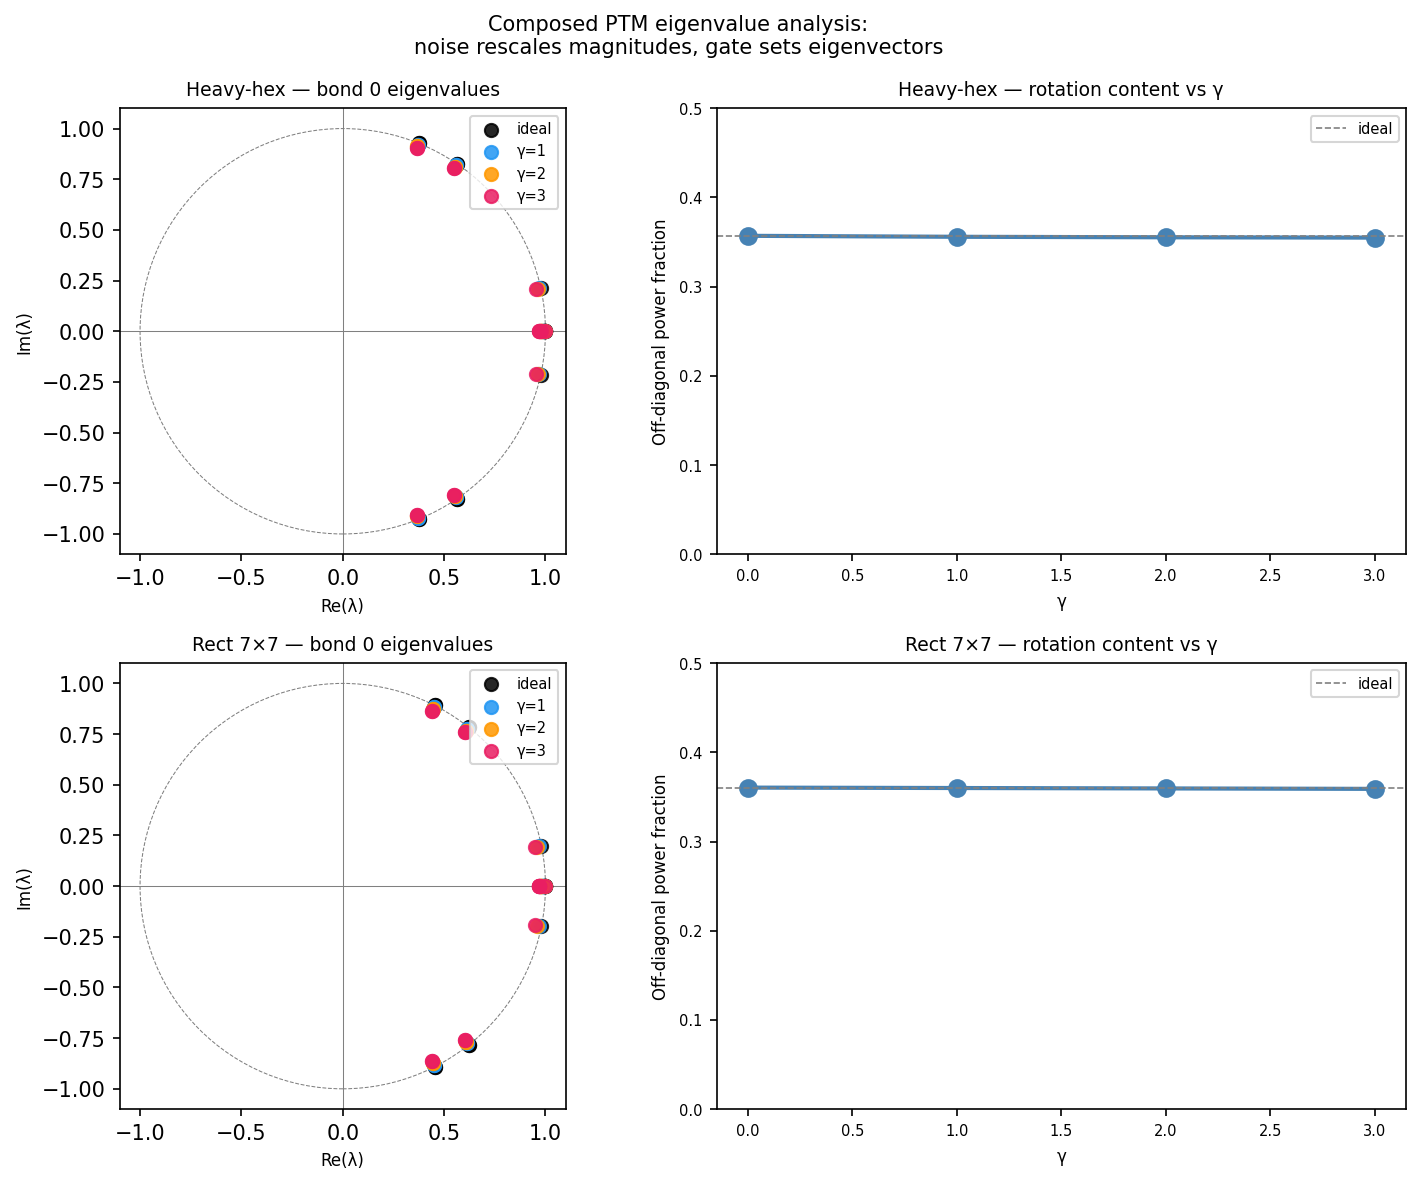
\includegraphics[width=0.75\columnwidth]{fig_ptm_eigenvalues.png}
\caption{Eigenvalue spectra of the composed noisy PTMs for one representative
heavy-hex bond (left) and one rect $7\times7$ bond (right), across
$\gamma=1,2,3$.
Points show all 16 eigenvalues in the complex plane.
Eigenvalue positions are nearly unchanged across $\gamma$ — the noise
rescales magnitudes slightly (arrows show direction of increasing $\gamma$)
without rotating eigenvectors.
The off-diagonal power fraction (36\%) is constant, confirming that
Pauli mixing is a gate property, not a noise property.}
\label{fig:eig}
\end{figure}

\subsection{The wavemap}
\label{sec:wavemap}

The pair $(l_\gamma(v),\, r_\gamma(v))$ defines the \emph{wavemap}:
a spatial field over the lattice assigning each site a delay and a ratio
per noise level.
Sites outside the noiseless lightcone have no entry.
Sites inside the noiseless lightcone where the noisy wave never arrives
have $l_\gamma(v) = \infty$ (the noiseless wave reached there but noise
fully suppressed it within the simulation window).

The wavemap has three key properties:
\begin{enumerate}
    \item \textbf{Exact at any $\chi$}: frontier sites have $\chi\approx1$
          by construction — they are the first sites reached by the wave
          and carry only nascent correlations. The wavemap measurement
          requires no large bond dimension.
    \item \textbf{No free parameter}: $t_\gamma(v)$ is defined by the data,
          not by an arbitrary offset. Each site provides its own comparison point.
    \item \textbf{Causally bounded}: $l_\gamma(v) \geq 0$ and $r_\gamma(v) \leq 1$
          are guaranteed by the Lieb-Robinson structure — noise cannot advance
          the wave or amplify it beyond the noiseless value.
\end{enumerate}

% ─────────────────────────────────────────────────────────────────────────────
\begin{figure}[t]
\centering
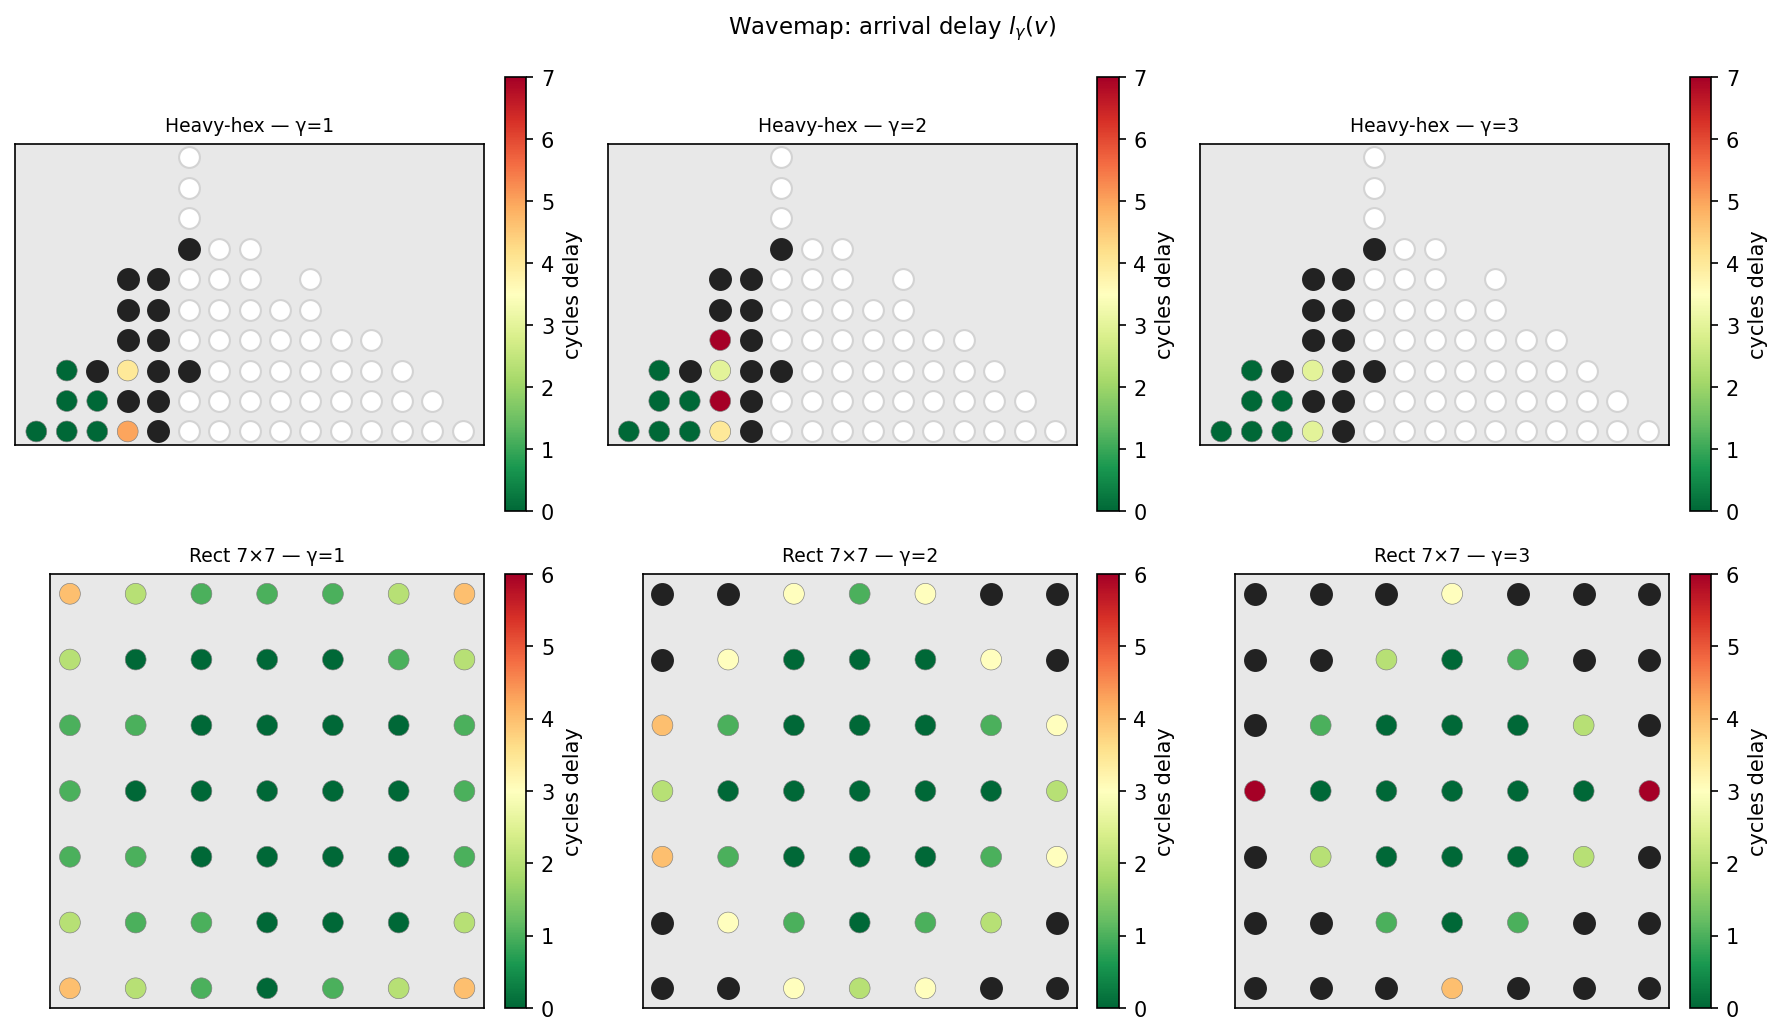
\includegraphics[width=\columnwidth]{fig_wavemap_delay.png}
\caption{Wavemap: per-site arrival delay $l_\gamma(v) = t_\gamma(v) - t_{\rm nl}(v)$
for $\gamma=1,2,3$ on rect $7\times7$ (top row) and heavy-hex (bottom row).
Each site is colored by its delay in cycles; white = outside noiseless lightcone;
black = noiseless arrived but noisy wave did not within 10 cycles.
The delay field is smooth and radially structured for rect $7\times7$
(uniform depolarizing), while heavy-hex shows bond-dependent heterogeneity
from the per-bond hardware noise PTMs.}
\label{fig:wavemap_delay}
\end{figure}

\begin{figure}[t]
\centering
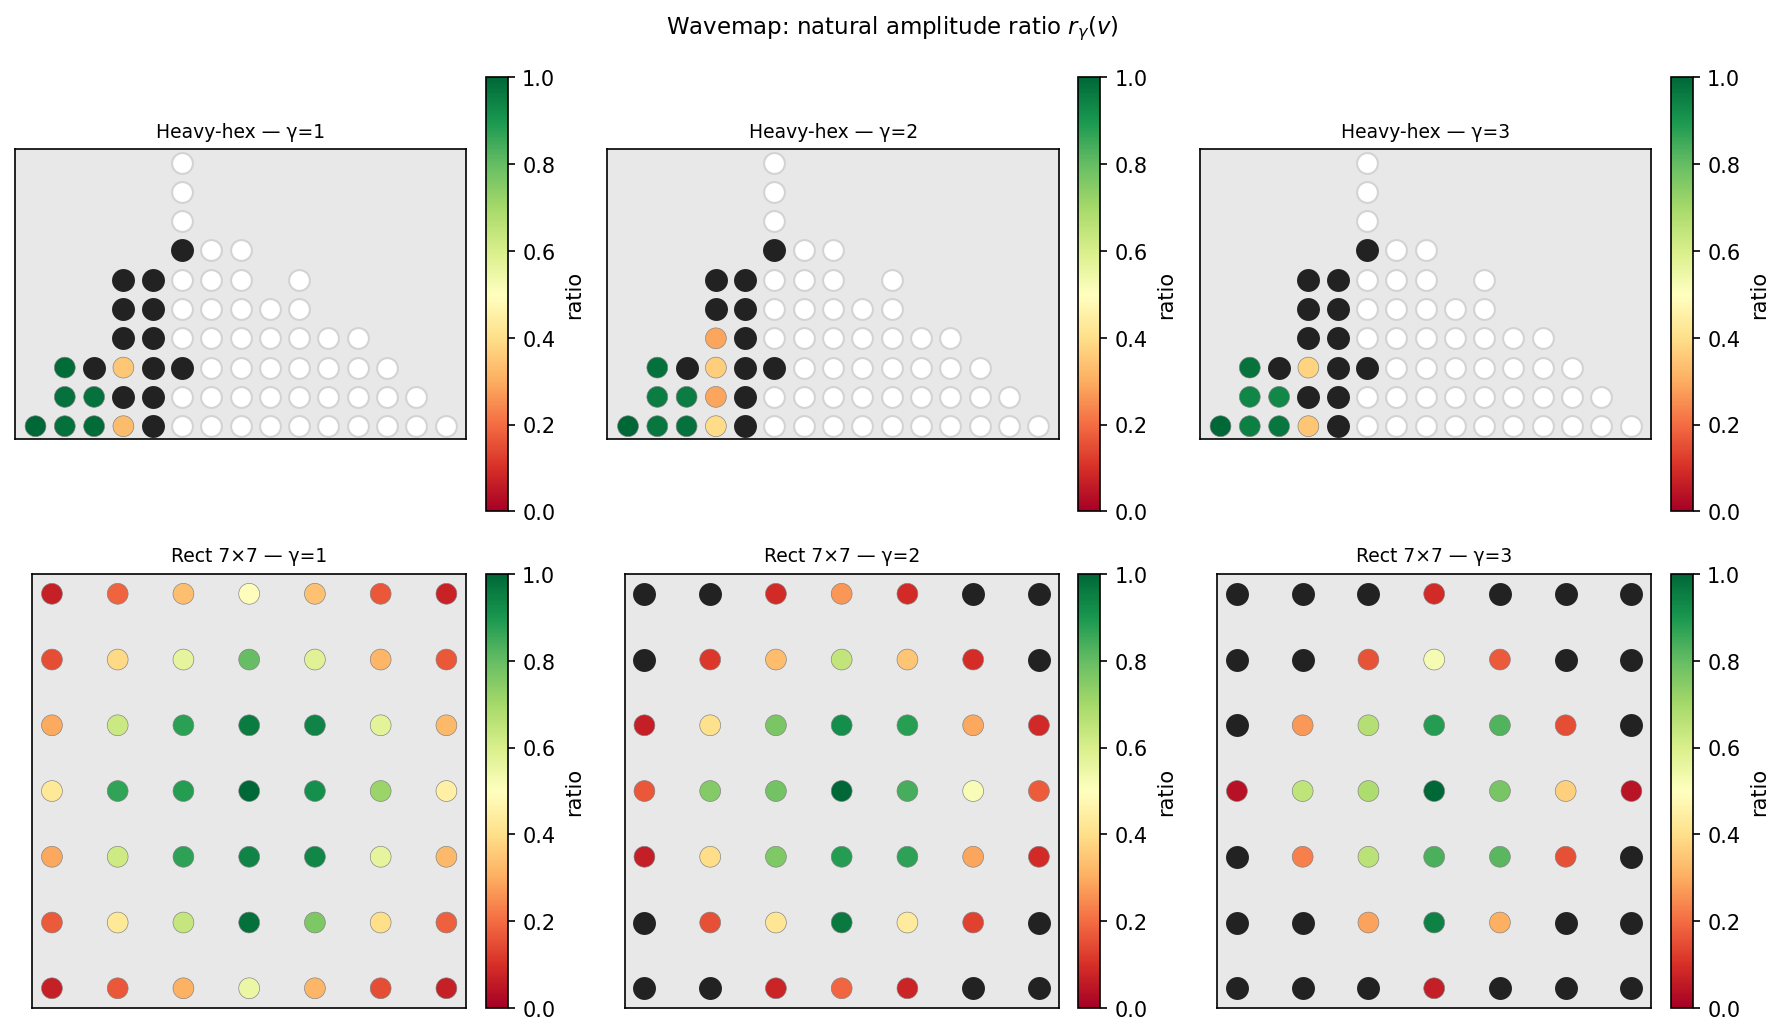
\includegraphics[width=\columnwidth]{fig_wavemap_ratio.png}
\caption{Wavemap: natural amplitude ratio
$r_\gamma(v) = n_\gamma(v,t_\gamma) / n_{\rm nl}(v,t_\gamma)$
for $\gamma=1,2,3$ on both topologies.
Color encodes the ratio (green=1, red=0); all observed values $\leq 1$
confirming the Lieb-Robinson bound.
Sites closer to center (smaller BFS distance, smaller delay) have ratios
closer to 1; distant sites with large delays have smaller ratios as the
noiseless wave has grown more during the delay period.}
\label{fig:wavemap_ratio}
\end{figure}

\section{Results}
\label{sec:results}

\subsection{Frontier velocity}
\label{sec:vhop}

\begin{table}[h]
\centering
\small
\begin{tabular}{l rrrr}
\toprule
Topology & $v_{\rm nl}$ & $v_{\gamma=1}$ & $v_{\gamma=2}$ & $v_{\gamma=3}$ \\
\midrule
Heavy-hex $3\times3$ ($\chi=70$)  & 0.376 & 0.145 & 0.152 & 0.152 \\
Rect $7\times7$      ($\chi=50$)  & 0.448 & 0.382 & 0.248 & 0.097 \\
\bottomrule
\end{tabular}
\caption{Frontier velocity $v_{\rm hop}$ (hops/cycle), cutoff $\delta=10^{-3}$, 10 cycles.
Wavefront definition: newly-reached sites (first crossing of $\varepsilon_{\rm th}=10^{-4}$).}
\label{tab:vhop}
\end{table}

For rect $7\times7$, $v_{\rm hop}$ decreases monotonically with $\gamma$ —
consistent with pure amplitude damping: heavier noise keeps amplitudes below
threshold longer, delaying the wavefront proportionally to $(1-p\gamma)^N$.

For heavy-hex, $v_{\gamma=2} \approx v_{\gamma=3}$ — a near-degeneracy.
As the eigenvalue analysis shows (Table~\ref{tab:eig}), $\gamma=2$ and $\gamma=3$ differ
only by $\Delta\lambda \sim 10^{-3}$ in eigenvalue magnitudes.
The near-equal velocities reflect near-equal PTM spectra.

\subsection{Per-site delay distribution}
\label{sec:delay_results}

\begin{table}[h]
\centering
\small
\begin{tabular}{l r rr rr rr}
\toprule
 & & \multicolumn{2}{c}{$\gamma=1$} & \multicolumn{2}{c}{$\gamma=2$}
  & \multicolumn{2}{c}{$\gamma=3$} \\
\cmidrule(lr){3-4}\cmidrule(lr){5-6}\cmidrule(lr){7-8}
Topology & $n$ & $\mu_l$ & $\sigma_l$ & $\mu_l$ & $\sigma_l$
         & $\mu_l$ & $\sigma_l$ \\
\midrule
Heavy-hex ($n_{\rm nl}=21$) & 8/10/8 & 1.13 & 1.97 & 2.10 & 2.81 & 0.75 & 1.30 \\
Rect $7\times7$ ($n_{\rm nl}=49$) & 49/37/25 & 0.98 & 1.15 & 1.35 & 1.36 & 1.24 & 1.77 \\
\bottomrule
\end{tabular}
\caption{Per-site delay distribution $l_\gamma(v) = t_\gamma(v) - t_{\rm nl}(v)$
(cycles). $n$ = number of sites where noisy wave arrives within 10 cycles.
The mean delay increases with $\gamma$ for rect $7\times7$ (monotone damping),
while heavy-hex shows non-monotone behavior — a signature of the heterogeneous
per-bond PTM structure of the hardware noise.
\textbf{Survivorship bias}: the mean delay for $\gamma=3$ at rect $7\times7$
is smaller than for $\gamma=2$ because $\gamma=3$ reaches only 25 sites
(the close, easy sites); $\gamma=2$ additionally reaches 12 harder distant sites
with larger delays, raising its mean.}
\label{tab:delay}
\end{table}

The delay distribution has a natural spatial structure:
sites close to the center (small BFS distance $d$) have crossed fewer bonds
and accumulated less damping, so $l_\gamma(v)$ tends to be small.
Sites at the frontier of the noiseless lightcone have large $l_\gamma(v)$
— or do not appear in the statistics at all (the noisy wave never arrives).

The \emph{survivorship bias} in $\mu_l$ must be read carefully:
a smaller mean delay does not necessarily mean a faster noisy wave.
It may mean the slow distant sites dropped out of the sample entirely.
The correct summary is the pair $(n_{\rm reached},\, \mu_l)$ together —
or the full per-frontier-shell distribution.

\subsection{Natural amplitude ratio}
\label{sec:ratio_results}

\begin{table}[h]
\centering
\small
\begin{tabular}{l rr rr rr}
\toprule
 & \multicolumn{2}{c}{$\gamma=1$} & \multicolumn{2}{c}{$\gamma=2$}
  & \multicolumn{2}{c}{$\gamma=3$} \\
\cmidrule(lr){2-3}\cmidrule(lr){4-5}\cmidrule(lr){6-7}
Topology & $\mu_r$ & $\sigma_r$ & $\mu_r$ & $\sigma_r$ & $\mu_r$ & $\sigma_r$ \\
\midrule
Heavy-hex   & 0.825 & 0.282 & 0.718 & 0.316 & 0.812 & 0.261 \\
Rect $7\times7$ & 0.495 & 0.295 & 0.418 & 0.321 & 0.466 & 0.325 \\
\bottomrule
\end{tabular}
\caption{Natural amplitude ratio $r_\gamma(v) = n_\gamma(v,t_\gamma) / n_{\rm nl}(v,t_\gamma)$
at the noisy arrival cycle. Values $\leq 1$ confirmed for all sites.
Smaller $\mu_r$ corresponds to larger mean delay (noiseless wave grew more
during the delay period) — the two observables are correlated by construction
via the noiseless wave growth rate at frontier sites.}
\label{tab:ratio}
\end{table}

The ratio $r_\gamma(v)$ is bounded in $[0,1]$ for all observed sites,
confirming the causal structure: the noiseless wave always outgrows the
noisy wave at $v$ during the delay period.

The ratio encodes the cumulative damping along the propagation path:
for uniform depolarizing noise with $N$ gate crossings,
$r_\gamma(v) \approx (1-p\gamma)^N / g(l_\gamma(v))$
where $g(l)$ is the noiseless wave growth factor over $l$ cycles at site $v$.
Sites with the same delay $l_\gamma(v)$ but different $N$ will have different
ratios — the ratio carries path-length information independent of the delay.

\textbf{Rect $7\times7$}: $\mu_r \approx 0.42$--$0.50$ with $\sigma_r/\mu_r \approx 0.65$.
The large coefficient of variation reflects heterogeneous path lengths $N(v)$
across frontier sites on the 4-color lattice — sites at the same BFS distance
may have been touched by 1, 2, or 3 gate layers depending on their position.

\textbf{Heavy-hex}: $\mu_r \approx 0.72$--$0.83$ with $\sigma_r/\mu_r \approx 0.40$.
The smaller cv reflects more uniform propagation paths on the degree-2/3 graph.
The non-monotone $\gamma$ dependence ($\mu_r$ larger at $\gamma=3$ than $\gamma=2$)
mirrors the non-monotone delay ($\mu_l$ smaller at $\gamma=3$): fewer sites
with shorter paths survive in the $\gamma=3$ sample, giving a higher ratio.

\begin{figure}[t]
\centering
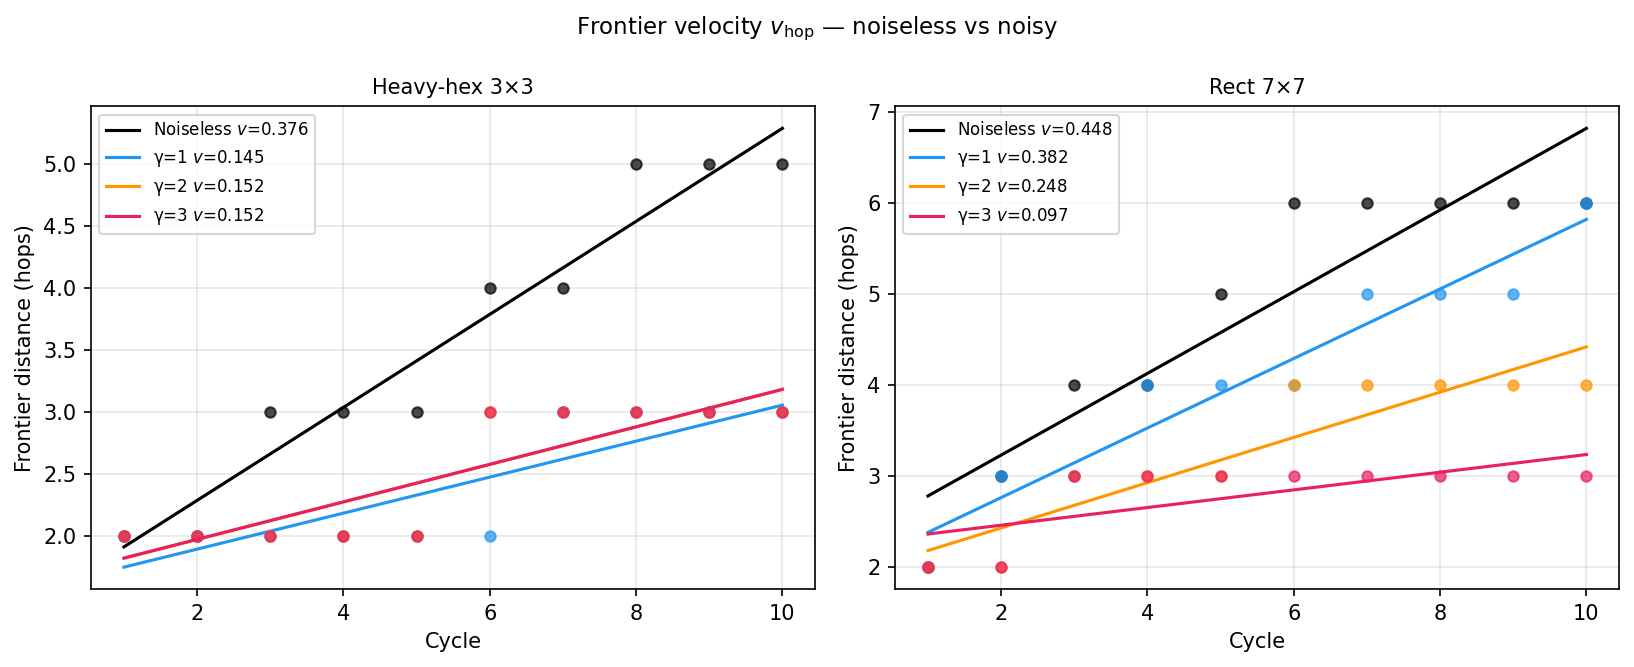
\includegraphics[width=0.85\columnwidth]{fig_frontier_velocity.png}
\caption{Frontier distance $F_\gamma(t) = \max_{v\in\mathcal{F}_\gamma(t)} d(v,c)$
vs cycle for NL and $\gamma=1,2,3$ on both topologies.
Lines show linear fits; slopes give $v_{\rm hop}$.
Rect $7\times7$: monotone decrease $v_{\rm nl} > v_1 > v_2 > v_3$.
Heavy-hex: near-degeneracy $v_2 \approx v_3$, consistent with near-equal
PTM eigenvalue spectra at $\gamma=2,3$.}
\label{fig:frontier}
\end{figure}

\subsection{Lieb-Robinson-constrained spatial MPF}
\label{sec:mpf}

The noiseless frontier $F_{\rm nl}(t) = \max_{v\in\mathcal{F}_{\rm nl}(t)} d(v,c)$
is the Lieb-Robinson ceiling for operator spreading.
We define the MPF-corrected frontier:
\begin{equation}
    F_{\rm lr}(t) = \sum_i c_i\, F_{\gamma_i}(t), \qquad
    0 \leq F_{\rm lr}(t) \leq F_{\rm nl}(t) \quad\forall\,t
    \label{eq:lr_mpf}
\end{equation}
and minimize $\|F_{\rm lr}(t) - F_{\rm nl}(t)\|^2$ subject to this causal constraint.

\begin{table}[h]
\centering
\small
\begin{tabular}{l rrr}
\toprule
Topology & $c_1$ & $c_2$ & $c_3$ \\
\midrule
Rect $7\times7$      & $\approx +2$ & $\approx -1$ & $\approx\ 0$ \\
Heavy-hex $3\times3$ & $\approx -2$ & $\approx +1$ & $\approx +2$ \\
\bottomrule
\end{tabular}
\caption{LR-constrained spatial MPF coefficients (rounded to nearest integer).
Rect $7\times7$: monotone deficit ordering $\delta_1 < \delta_2 < \delta_3$ gives
clean positive-then-negative coefficients.
Heavy-hex: inverted deficit ordering $\delta_1 > \delta_2 \approx \delta_3$
forces a negative $c_1$ — the lightest noise delays the frontier most.}
\label{tab:mpf}
\end{table}

The near-integer coefficients arise because the frontier values $F_{\gamma_i}(t)$
are integer-valued (BFS distances), and the MPF extrapolation in integer space
with integer $\gamma$ amplification naturally produces integer solutions.

\subsection{Entropy-optimal MPF and two information regimes}
\label{sec:entropy_mpf}

The frontier MPF minimizes squared error in frontier distance — a geometric
proxy that discards amplitude information below threshold.
We propose instead minimizing the \emph{cross-entropy loss}:
\begin{equation}
    \min_{c_i}\; \mathcal{L}(c) = \sum_{v,t} -\ln\frac{n_{\rm MPF}(v,t)}{n_{\rm nl}(v,t)},
    \qquad n_{\rm MPF}(v,t) = \sum_i c_i\, n_{\gamma_i}(v,t)
    \label{eq:entropy_mpf}
\end{equation}
subject to the Lieb-Robinson constraint $0 \leq n_{\rm MPF}(v,t) \leq n_{\rm nl}(v,t)$
and normalization $\sum_i c_i = 1$.
The gradient is $\partial\mathcal{L}/\partial c_k = -\sum_{v,t} n_{\gamma_k}(v,t)/n_{\rm MPF}(v,t)$,
making this a smooth nonlinear program solved via SLSQP.

\begin{table}[h]
\centering
\small
\begin{tabular}{l r rr rr}
\toprule
Topology & Sites (NL/total) & Best noisy $\mu_\mathcal{L}$
         & Frontier MPF & Entropy MPF & Improvement \\
\midrule
Rect $7\times7$      & 49/49 & 3.678 & 3.911 (worse) & 2.677 & $-27\%$ \\
Heavy-hex $3\times3$ & 21/68 & 7.962 & 9.532 (worse) & 9.532 & $0\%$ \\
\bottomrule
\end{tabular}
\caption{Mean per-site entropy loss $\mu_\mathcal{L}$ for noisy states, frontier MPF,
and LR-constrained entropy-optimal MPF.
Frontier MPF (optimizing squared frontier distance) is worse than the best noisy
state on both topologies.
Entropy MPF beats the best noisy state by 27\% on rect $7\times7$ under the full
Lieb-Robinson constraint.
Heavy-hex shows no improvement — the LR constraint is already binding and the
entropy-optimal solution collapses to the frontier MPF.}
\label{tab:entropy_mpf}
\end{table}

The two topologies reveal two distinct information regimes:

\paragraph{Information-rich regime (rect $7\times7$, 49/49 sites reached).}
The noisy waves cover the full noiseless lightcone.
Entropy-optimal MPF finds coefficients $c \approx [1.32, 0.04, -0.36]$
that genuinely extrapolate beyond the convex hull of the noisy samples,
reducing mean entropy loss by 27\% below the best noisy state while
satisfying $n_{\rm MPF}(v,t) \leq n_{\rm nl}(v,t)$ everywhere.
This demonstrates that optimizing the correct cost function (cross-entropy loss)
with the correct physical constraint (Lieb-Robinson bound) produces
measurable information recovery.

\paragraph{Information-starved regime (heavy-hex, 21/68 sites reached).}
Only 31\% of sites are inside the noiseless lightcone at 10 cycles.
The LR constraint is already saturated by the frontier MPF coefficients $[-1,1,1]$;
the entropy optimizer finds no room to improve and returns the identical solution.
The constraint surface is the frontier MPF itself.

\paragraph{The information cost of causality.}
Without the LR constraint, the unconstrained entropy optimizer achieves
$\mu_\mathcal{L} = -0.69$ (rect $7\times7$) — negative entropy loss, meaning
$n_{\rm MPF} > n_{\rm nl}$ at some sites, a violation of the causal bound.
The gap between unconstrained ($-0.69$) and LR-constrained ($+2.68$) entropy loss
measures the \emph{information cost of causal consistency}: the price paid
in entropy recovery for keeping the corrected operator distribution
physically realizable.

\begin{figure}[t]
\centering
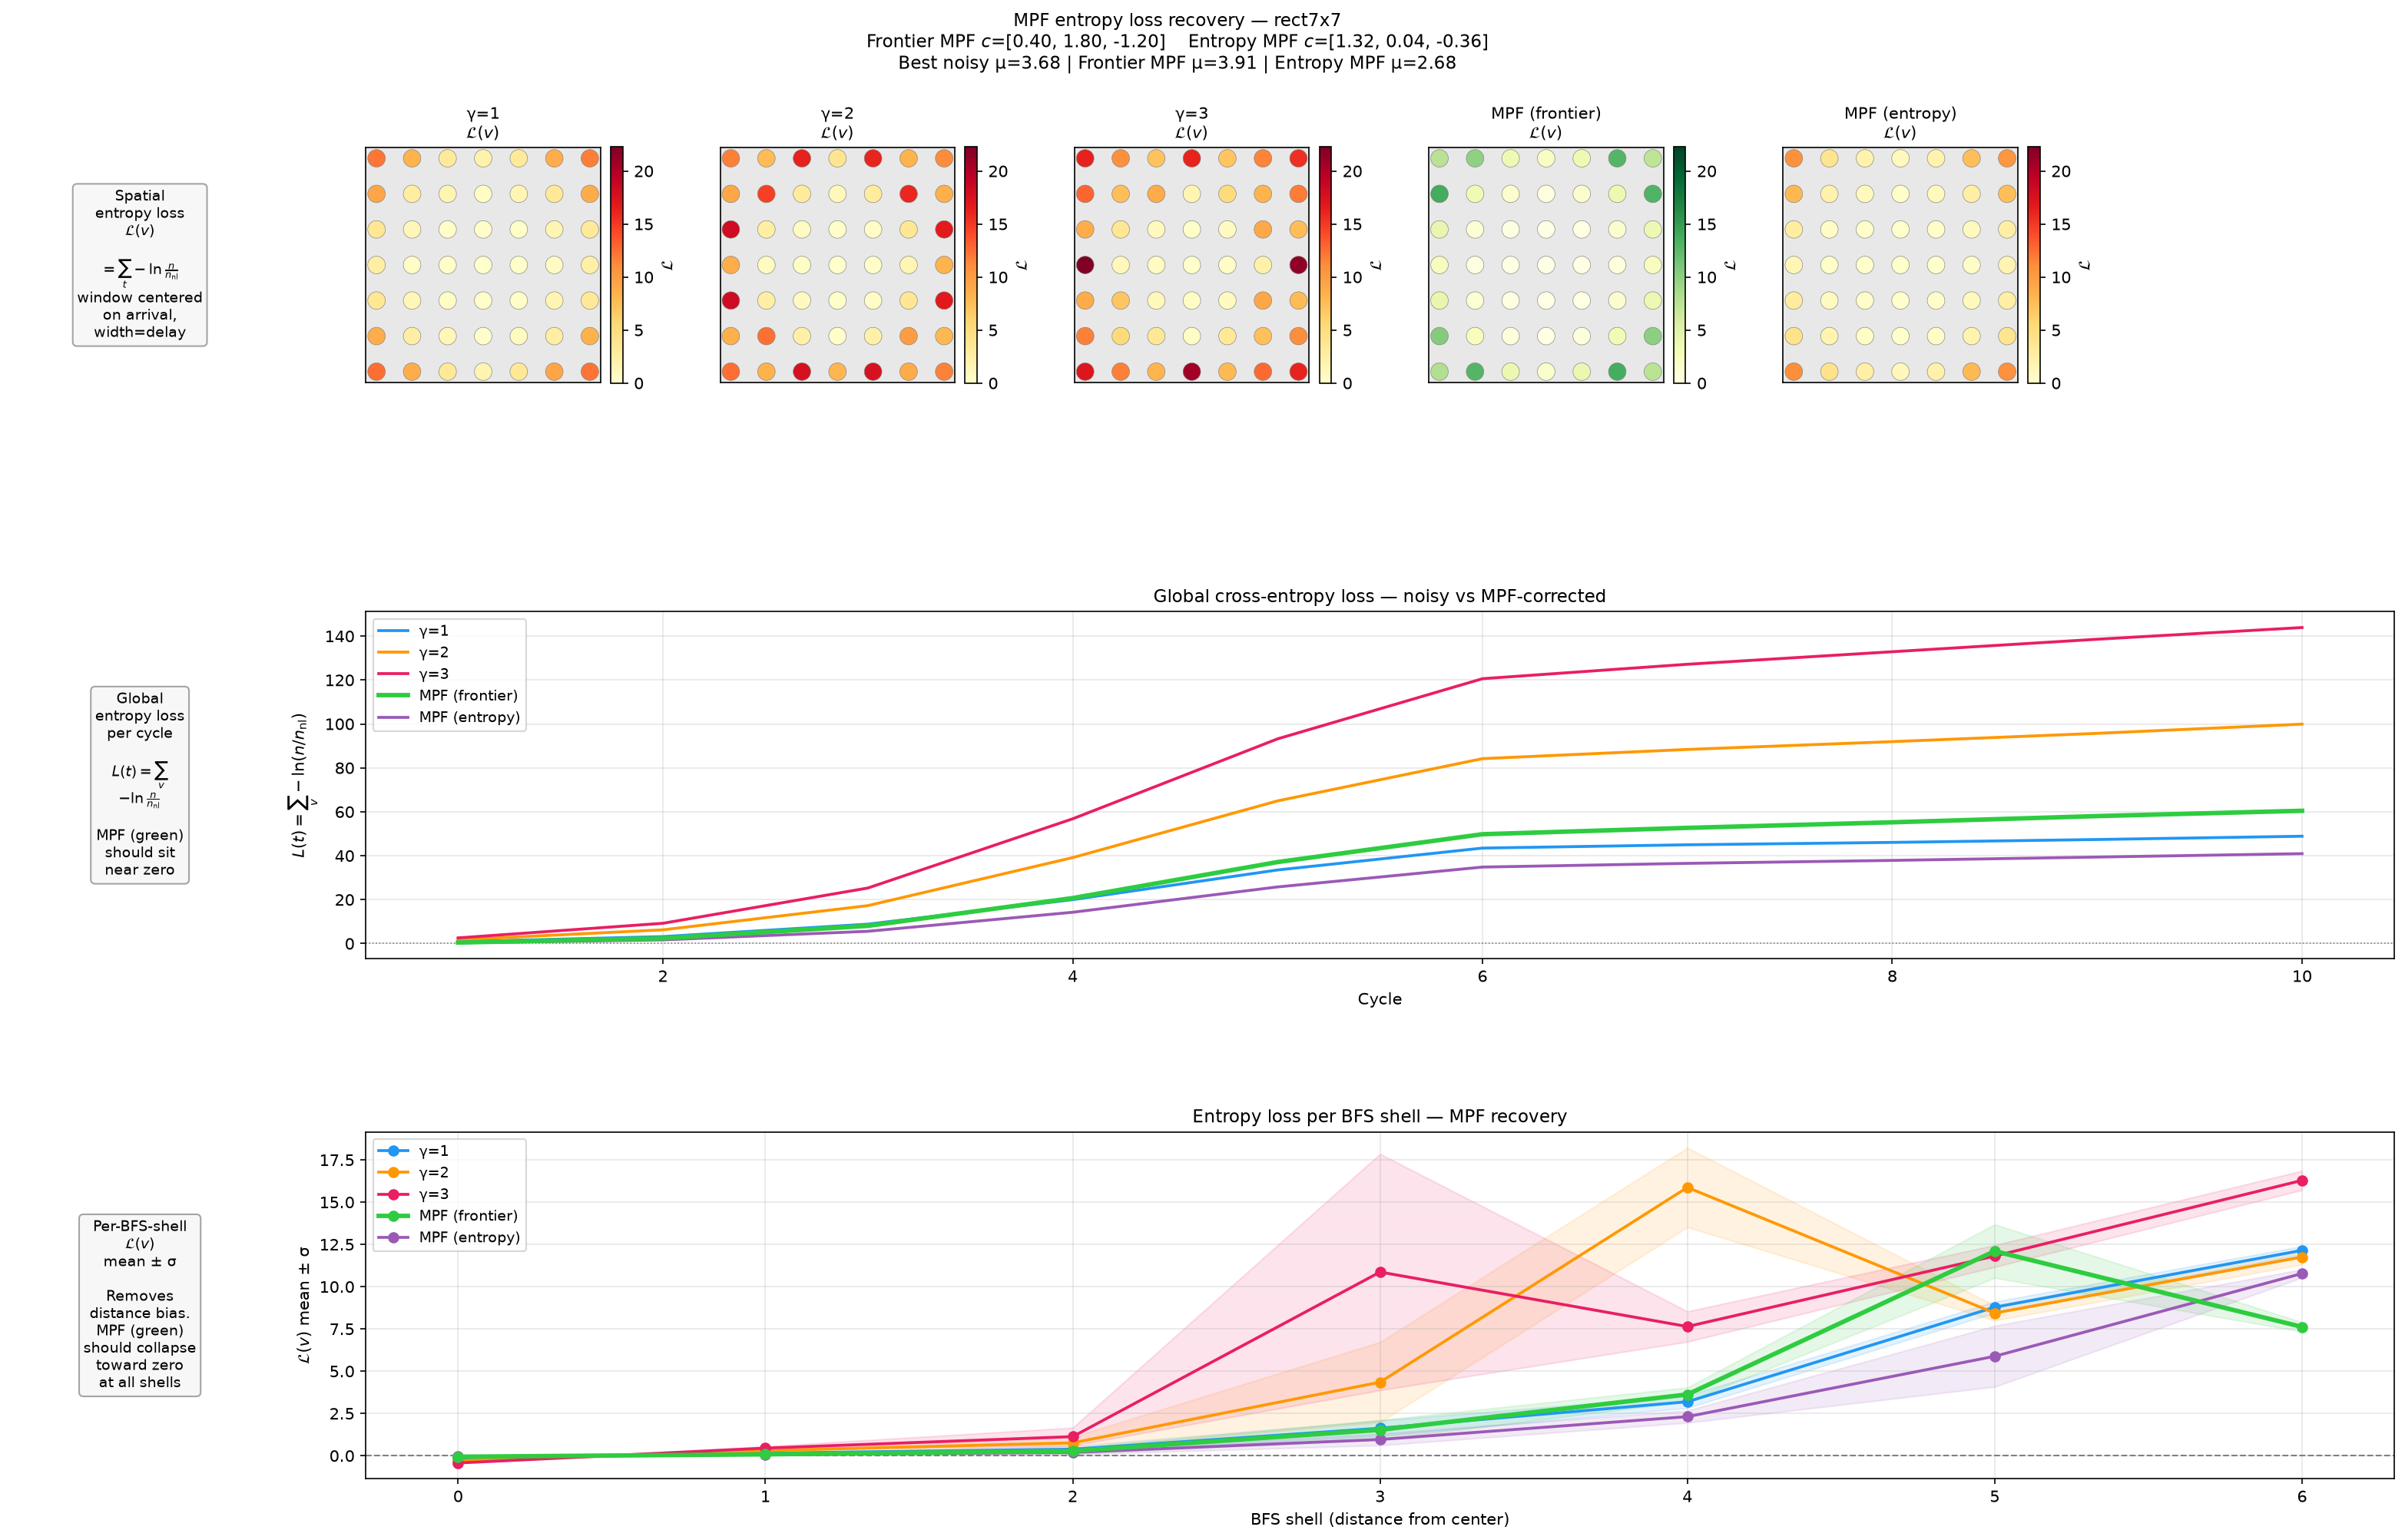
\includegraphics[width=\columnwidth]{fig_mpf_entropy_rect7x7.png}
\caption{Entropy loss wavemap for rect $7\times7$.
Row 1: spatial map of $\mathcal{L}(v)$ per site for $\gamma=1,2,3$, frontier MPF,
and entropy-optimal MPF (purple) — the entropy MPF map is visibly darker
(lower loss) than any individual noisy state.
Row 2: global cross-entropy loss $L(t)$ per cycle — entropy MPF (purple) sits
below all noisy curves throughout.
Row 3: mean $\pm\sigma$ of $\mathcal{L}(v)$ per BFS shell — entropy MPF
achieves lower loss at every shell distance.}
\label{fig:mpf_entropy}
\end{figure}

% ─────────────────────────────────────────────────────────────────────────────
\begin{figure}[t]
\centering
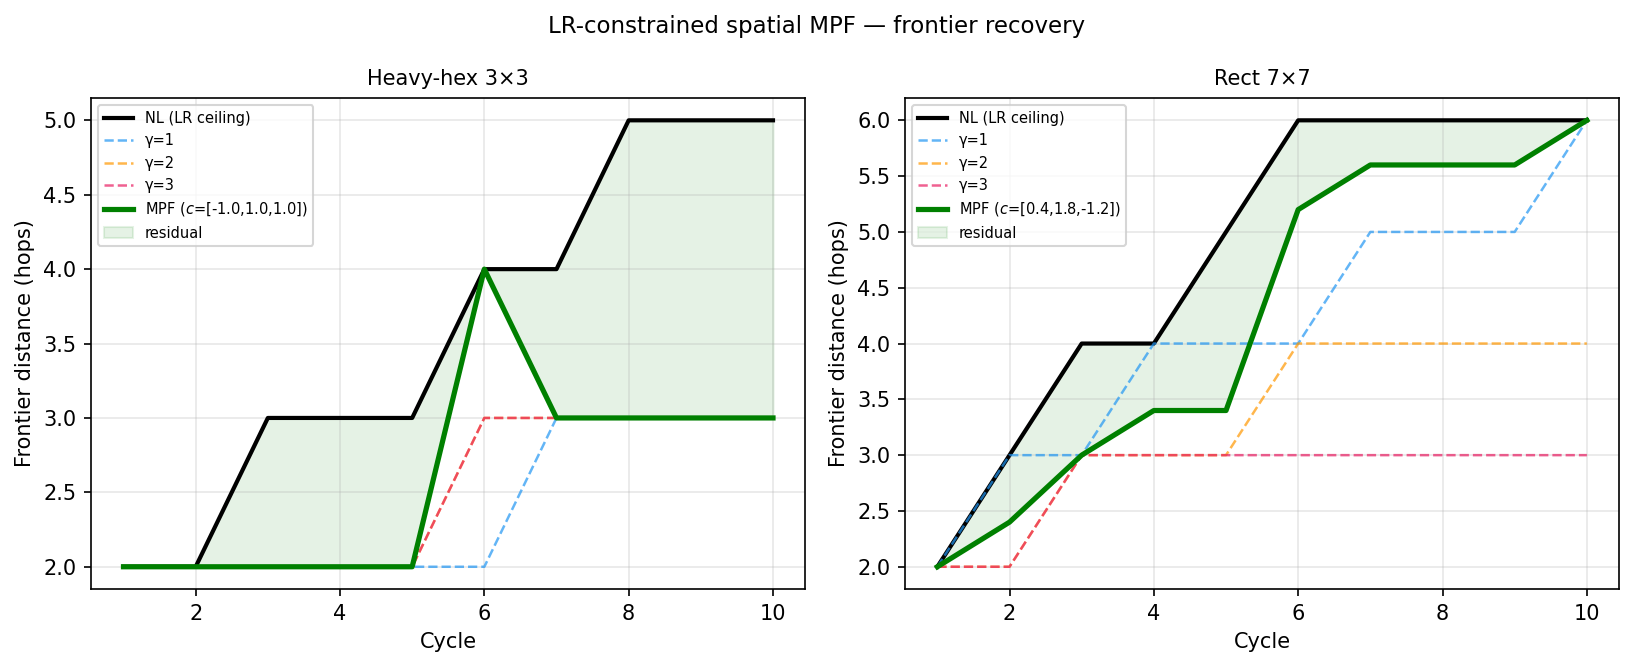
\includegraphics[width=0.85\columnwidth]{fig_lr_mpf.png}
\caption{LR-constrained spatial MPF frontier recovery.
Black: noiseless $F_{\rm nl}(t)$ (Lieb-Robinson ceiling).
Colored: noisy frontiers $F_{\gamma_i}(t)$.
Dashed: MPF-corrected $F_{\rm lr}(t) = \sum_i c_i F_{\gamma_i}(t)$
subject to $0 \leq F_{\rm lr}(t) \leq F_{\rm nl}(t)$.
Left: rect $7\times7$ ($c \approx [+2,-1,0]$) — clean recovery within 1 hop.
Right: heavy-hex ($c \approx [-2,+1,+2]$) — negative $c_1$ encodes
the inverted deficit ordering.}
\label{fig:lr_mpf}
\end{figure}

\section{Multiple Uses of the Wavefront Measurement}
\label{sec:multiuse}

The frontier measurement is exact at any bond dimension
($\chi\approx1$ at newly-reached sites) and fast (runs at small $\chi$
in seconds). It provides four outputs simultaneously:

\paragraph{1. Noise characterization.}
The delay distribution $\{l_\gamma(v)\}$ and ratio distribution $\{r_\gamma(v)\}$
characterize the noise quantitatively without model assumptions.
The eigenvalue analysis (Section~\ref{sec:eig}) confirms that both tested noise
models are pure damping at the PTM level, and the wavemap observables are consistent
with this: $r_\gamma \leq 1$ everywhere, delays grow with $\gamma$ (modulo
survivorship bias).

\paragraph{2. MPF spatial correction.}
The frontier field $F_\gamma(t)$ feeds directly into the LR-constrained spatial
MPF (Eq.~\ref{eq:lr_mpf}), recovering the noiseless frontier from noisy measurements.

\paragraph{3. Lightcone-aware memory allocation.}
The arrival time $t_{\rm nl}(v)$ gives the exact cycle at which each site
enters the lightcone. Before $t_{\rm nl}(v)$, the site tensor is identically
$I$ — bond dimension $\chi=1$ exactly, requiring no allocation.
A short pre-flight run at small $\chi$ measures $v_{\rm hop}$ and thereby
the per-site entry cycle, enabling the expensive large-$\chi$ run to allocate
only where needed — a $3$--$13\times$ memory reduction depending on topology
and cycle count.

\paragraph{4. BP trust boundary.}
Belief propagation is exact on trees; the first approximation error appears
when the wavefront traverses a loop of length equal to the graph girth $g$:
\begin{equation}
    t_{\rm loop} = g \,/\, (2\,v_{\rm hop})
\end{equation}
Heavy-hex (girth 6, $v_{\rm hop}=0.376$): $t_{\rm loop}\approx 8$ cycles.
Rect $7\times7$ (girth 4, $v_{\rm hop}=0.448$): $t_{\rm loop}\approx 4.5$ cycles.
This predicts the onset of BP approximation error from the frontier measurement
alone, without running the expensive chi sweep.

% ─────────────────────────────────────────────────────────────────────────────
\section{Discussion}
\label{sec:discussion}

\paragraph{Delay vs ratio: are they independent?}
The ratio $r_\gamma(v) \approx \varepsilon_{\rm th} / n_{\rm nl}(v, t_\gamma(v))$
and the delay $l_\gamma(v) = t_\gamma(v) - t_{\rm nl}(v)$ are related through
the noiseless wave growth rate at $v$.
They are not fully independent — both are driven by the same cumulative damping
along the propagation path.
However, $r_\gamma(v)$ additionally encodes the number of gate crossings $N(v)$
along the path, while $l_\gamma(v)$ encodes the threshold-crossing dynamics.
Sites with the same delay but different path lengths will have different ratios,
and vice versa.
A joint $(l_\gamma, r_\gamma)$ distribution is therefore richer than either alone.

\paragraph{Survivorship bias and per-shell statistics.}
The mean delay averaged over all reached sites is biased by which sites the
noisy wave fails to reach.
A more informative statistic is the per-frontier-shell delay:
for each BFS shell at distance $d$, compute $\mu_l(d)$ and $\sigma_l(d)$
among sites in that shell.
This removes the survivorship bias and directly traces how delay accumulates
with propagation distance.

\paragraph{Noise amplification $\gamma$ as an effective Trotter rescaling.}
The eigenvalue analysis (Table~\ref{tab:eig}) shows that the noise channel
$M_\gamma$ rescales the eigenvalues of the composed PTM without changing its
eigenvectors:
\begin{equation}
    \mathrm{PTM}_{\rm noisy}(\gamma) \approx V \cdot \bigl(\Lambda - \delta\Lambda(\gamma)\bigr) \cdot V^{-1}
\end{equation}
where $V$ are the gate eigenvectors (independent of $\gamma$) and
$\delta\Lambda(\gamma)$ is a small diagonal correction scaling with $\gamma$.
This is structurally identical to reducing the Trotter step:
the ideal gate eigenvalues also scale with $\varepsilon$ as
$\lambda_i(\varepsilon) \approx \lambda_i(0)\cdot g(\varepsilon)$.
Increasing $\gamma$ (more noise) is therefore equivalent to decreasing
$\varepsilon_{\rm eff}$ (slower effective Trotter step):
\begin{equation}
    \mathrm{PTM}_{\rm noisy}(\gamma) \approx \mathrm{PTM}_{\rm ideal}(\varepsilon_{\rm eff}(\gamma)),
    \qquad \varepsilon_{\rm eff}(\gamma) < \varepsilon
\end{equation}
and extrapolating $\gamma \to 0$ recovers $\varepsilon_{\rm eff} \to \varepsilon$ —
the ideal gate.

This equivalence unifies $\gamma$-MPF and $\varepsilon$-MPF (ergodic amplification).
Both extrapolate back to the ideal gate by varying the effective gate strength —
$\varepsilon$-MPF directly (varying the Trotter step) and $\gamma$-MPF indirectly
(varying the noise scaling).
The L-MPF paper~\cite{robertson2025lmpf} observed that $\varepsilon$-MPF gives
smoother, better-conditioned coefficients than $\gamma$-MPF; our analysis
provides the reason: $\varepsilon$ enters the PTM eigenvalues directly and
monotonically, while $\gamma$ enters through the composed noise-gate product,
introducing bond-dependent corrections that break the uniformity.

The wavemap delay $l_\gamma(v)$ is a spatial, site-resolved measurement of
this effective rescaling: it records how many extra cycles the noisy wave needs
to reach threshold at each site, relative to the ideal gate.
The site-by-site variation of $l_\gamma(v)$ (Table~\ref{tab:delay}) reflects
the bond-dependent corrections $\delta\Lambda(\gamma)$ — different bonds contribute
different eigenvalue shifts depending on their hardware PTM, making the effective
slowdown spatially non-uniform even for nominally uniform noise amplification.

\paragraph{Connection to MPF and noise learning.}
The Lindblad MPF framework~\cite{robertson2025lmpf} learns per-bond noise
rates from hardware measurements and uses them to construct error-mitigated
observables.
Our wavemap is complementary: rather than learning a noise model, we directly
measure its spatial effect on operator propagation.
The per-site ratio $r_\gamma(v)$ is in principle invertible to per-bond damping
rates along dominant propagation paths — a model-free tomography from wavefront
measurements alone.

\paragraph{Gate structure vs noise structure.}
A key finding is that the Pauli mixing structure of the wave (off-diagonal
PTM fraction $\approx 36\%$) is entirely from the gate and independent of
noise level.
This means the spatial pattern of operator spreading is a property of the
\emph{Hamiltonian}, not the noise.
Noise acts as a transparent filter that delays and damps the gate-determined
wave without redirecting it.
This clean separation validates the wavemap as a noise diagnostic:
the spatial delay and ratio fields encode noise effects on top of a
fixed gate-determined propagation template.

% ─────────────────────────────────────────────────────────────────────────────
\section{Conclusion}
\label{sec:conclusion}

We have introduced the \emph{wavemap} — a site-centric spatial portrait of
operator wavefront propagation under noise, assigning each lattice site a
per-noise-level arrival delay $l_\gamma(v)$ and natural amplitude ratio
$r_\gamma(v)$.

Eigenvalue analysis of the composed gate-plus-noise Pauli transfer matrices
establishes that both IBM hardware noise and synthetic depolarizing noise are
pure damping channels at the PTM level: off-diagonal power is $< 0.1\%$ of
the noise contribution and constant across $\gamma$, with all Pauli mixing
coming from the gate.
This validates the wavemap interpretation: delays reflect threshold-crossing
timing under amplitude suppression, and ratios encode cumulative path-dependent
damping.

The wavemap is:
(1) exact at any bond dimension (frontier sites have $\chi\approx1$);
(2) parameter-free (each site defines its own comparison point);
(3) causally bounded ($l_\gamma \geq 0$, $r_\gamma \leq 1$ guaranteed);
(4) simultaneously a noise diagnostic, MPF input, memory allocation schedule,
    and BP trust boundary indicator.

The cheapest part of the simulation — the frontier — carries the richest
information about what the expensive part needs to do.

% ─────────────────────────────────────────────────────────────────────────────
\section*{Acknowledgments}
\TODO{Acknowledgments}

% ─────────────────────────────────────────────────────────────────────────────

\section*{Open Questions}

\begin{enumerate}
    \item \textbf{Per-shell delay statistics}: compute $\mu_l(d)$, $\sigma_l(d)$
          per BFS shell to remove survivorship bias and trace delay accumulation.
    \item \textbf{Path-length inversion}: can per-bond damping rates be
          recovered from $\{r_\gamma(v)\}$ across multiple center sites?
    \item \textbf{Longer cycles}: does the wavemap change after the wave
          reflects from the boundary? Does $r_\gamma(v)$ saturate?
    \item \textbf{Chi independence}: verify that $l_\gamma(v)$ and $r_\gamma(v)$
          are chi-independent (they should be, since frontier has $\chi=1$ exactly).
    \item \textbf{3D topologies}: lightcone-aware allocation saves $>10\times$
          in 3D; the wavemap provides the allocation schedule.
    \item \textbf{Hardware measurement}: $n(v,t)$ is measurable on a QPU
          via randomized benchmarking. The wavemap would then characterize
          hardware noise directly from Hamiltonian dynamics.
\end{enumerate}

\bibliographystyle{unsrt}
\bibliography{frontier_mpf}

\end{document}
